% ------------------------------------------------------------------------------
% TYPO3 CMS 7.5 - What's New - Chapter "Introduction" (Spanish Version)
%
% @author	Michael Schams <schams.net>
% @license	Creative Commons BY-NC-SA 3.0
% @link		http://typo3.org/download/release-notes/whats-new/
% @language	Spanish
% ------------------------------------------------------------------------------
% LTXE-CHAPTER-UID:		3a84d600-9fb67dda-31c4af65-dd7a4af5
% LTXE-CHAPTER-NAME:	Introduction
% ------------------------------------------------------------------------------

\section{Introducción}
\begin{frame}[fragile]
	\frametitle{Introducción}

	\begin{center}\huge{Introducción}\end{center}
	\begin{center}\huge{\color{typo3darkgrey}\textbf{Los Hechos}}\end{center}

\end{frame}

% ------------------------------------------------------------------------------
% LTXE-SLIDE-START
% LTXE-SLIDE-UID:		3507b7a6-7725ae95-259f1c3c-018dc51f
% LTXE-SLIDE-ORIGIN:	81d53787-fb3806f0-841b4042-7033fad4 English
% LTXE-SLIDE-ORIGIN:	f1ea1041-2b6b2b81-f54b45c0-84265d6a German
% LTXE-SLIDE-TITLE:		TYPO3 CMS 7.5 - The Facts
% ------------------------------------------------------------------------------
\begin{frame}[fragile]
	\frametitle{Introducción}
	\framesubtitle{TYPO3 CMS 7.5 - Los Hechos}

	\begin{itemize}
		\item Fecha de lanzamiento: 29 Septiembre 2015
		\item Tipo de lanzamiento: "Lanzamiento Sprint"
		\item Visión: Adoptar, Innovar, Lanzar
		\item Foco principal: Finalización
	\end{itemize}

	\begin{figure}
		
\includegraphics[width=0.95\linewidth]{Introduction/typo3cms75-banner.jpg}
	\end{figure}

\end{frame}

% ------------------------------------------------------------------------------
% LTXE-SLIDE-START
% LTXE-SLIDE-UID:		ffc3241e-bb6fb540-600149ef-6cbbc825
% LTXE-SLIDE-ORIGIN:	a0327db8-b4a9bd42-f32515d0-87296684 English
% LTXE-SLIDE-ORIGIN:	5d8adc7d-af29cb46-4acd2255-27362935 German
% LTXE-SLIDE-TITLE:		System Requirements
% ------------------------------------------------------------------------------
\begin{frame}[fragile]
	\frametitle{Introducción}
	\framesubtitle{Requisitos del Sistema}

	\begin{itemize}
		\item PHP*:\tabto{2.2cm}v5.5.0 - v5.6.x
		\item MySQL:\tabto{2.2cm}v5.5.x - v5.6.x (modo no estricto)
		\item Espacio de disco:\tabto{3.4cm}mín 200 MB
		\item Ajustes de PHP:

			\begin{itemize}
				\item memory\_limit >= 128M
				\item max\_execution\_time >= 240s
				\item opción de compilación \texttt{--disable-ipv6} \underline{no} debe ser usada
			\end{itemize}

		\item Backend requiere IE >= 9 o cualquier otro navegador moderno

	\end{itemize}

	\vspace{1cm}

	*) Detalles adicionales: \href{http://typo3.org/news/article/php-minimum-requirements-for-typo3-cms-7/}{Requisitos Mínimos de PHP para TYPO3 CMS 7}

\end{frame}

% ------------------------------------------------------------------------------
% LTXE-SLIDE-START
% LTXE-SLIDE-UID:		4f59e651-3fa1b31f-bdb17b74-57ad4789
% LTXE-SLIDE-ORIGIN:	c155d534-1a53682d-f56423dc-163111d3 English
% LTXE-SLIDE-ORIGIN:	6cad14bf-08874e74-1dd85333-e5c43a08 German
% LTXE-SLIDE-TITLE:		Development And Release Timeline
% ------------------------------------------------------------------------------
\begin{frame}[fragile]
	\frametitle{Introducción}
	\framesubtitle{Línea de tiempo de Desarrollo y Lanzamiento}

	\begin{figure}
		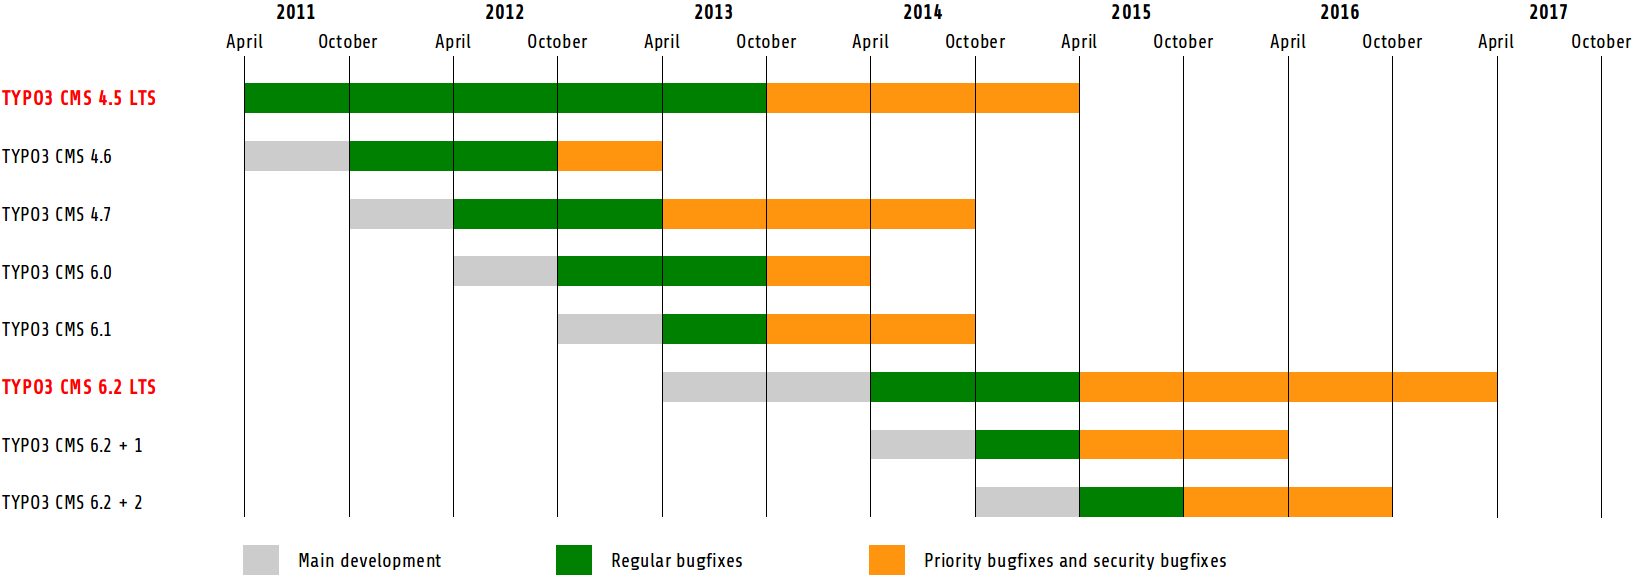
\includegraphics[width=0.90\linewidth]{Introduction/ReleaseAgenda.png}
	\end{figure}

\end{frame}

% ------------------------------------------------------------------------------
% LTXE-SLIDE-START
% LTXE-SLIDE-UID:		94c3cc1b-09f07e33-6bc803c4-1c9b23f9
% LTXE-SLIDE-ORIGIN:	83c1fb1c-ed592fa9-a2a279bd-be5cc800 English
% LTXE-SLIDE-ORIGIN:	387f7aeb-53ab533f-95427547-3aa76412 German
% LTXE-SLIDE-TITLE:		TYPO3 CMS Roadmap
% ------------------------------------------------------------------------------
\begin{frame}[fragile]
	\frametitle{Introducción}
	\framesubtitle{Línea de lanzamiento de TYPO3 CMS}

	Fechas de lanzamiento estimadas y sus enfoques principales:

	\begin{itemize}
		\item v7.0 \tabto{1.1cm}02/Dic/2014\tabto{3.4cm}Revisión de Backend Vol 1
		\item v7.1 \tabto{1.1cm}24/Feb/2015\tabto{3.4cm}Optimización \& Limpieza del núcleo
		\item v7.2 \tabto{1.1cm}28/Apr/2015\tabto{3.4cm}Frontend
		\item v7.3 \tabto{1.1cm}16/Jun/2015\tabto{3.4cm}Ecosistema de Paquetes, Composer\newline
			\tabto{3.4cm}y Manejo de Extensiones
		\item v7.4 \tabto{1.1cm}04/Ago/2015\tabto{3.4cm}Revisión de Backend Vol 2

		\item
			\begingroup
				\color{typo3orange}
					v7.5 \tabto{1.1cm}29/Sep/2015\tabto{3.4cm}Finalización
			\endgroup

		\item v7 LTS \tabto{1.1cm}Oct/Nov/2015\tabto{3.4cm}\textbf{TYPO3 CMS 7 LTS} (Lanzamiento a Largo Plazo)
	\end{itemize}

	\smaller
		\url{https://typo3.org/typo3-cms/roadmap/}\newline
		\url{http://typo3.org/news/article/embrace-and-innovate-typo3-cms-7/}
	\normalsize

\end{frame}

% ------------------------------------------------------------------------------
% LTXE-SLIDE-START
% LTXE-SLIDE-UID:		f031e20e-7682f204-9cd0c8cf-8767e846
% LTXE-SLIDE-ORIGIN:	63decc15-57478e30-70c7ae99-27abd3c2 English
% LTXE-SLIDE-ORIGIN:	3b01edfd-6f06e241-2670b2ad-1b598b4e German
% LTXE-SLIDE-TITLE:		Installation
% ------------------------------------------------------------------------------
\begin{frame}[fragile]
	\frametitle{Introducción}
	\framesubtitle{Instalación}

	\begin{itemize}
		\item Procedimiento de instalación oficial bajo Linux/Mac OS X\newline
			(DocumentRoot por ejemplo \texttt{/var/www/site/htdocs}):
		\begin{lstlisting}
			$ cd /var/www/site
			$ wget --content-disposition get.typo3.org/7.5
			$ tar xzf typo3_src-7.5.0.tar.gz
			$ cd htdocs
			$ ln -s ../typo3_src-7.5.0 typo3_src
			$ ln -s typo3_src/index.php
			$ ln -s typo3_src/typo3
			$ touch FIRST_INSTALL
		\end{lstlisting}

		\item Enlaces simbólicos bajo Microsoft Windows:

			\begin{itemize}
				\item Use \texttt{junction} en Windows XP/2000
				\item Use \texttt{mklink} en Windows Vista y Windows 7
			\end{itemize}

	\end{itemize}
\end{frame}

% ------------------------------------------------------------------------------
% LTXE-SLIDE-START
% LTXE-SLIDE-UID:		07506796-e33d55f7-af59279f-6b5a1758
% LTXE-SLIDE-ORIGIN:	4dbfb1f2-70930473-ec804474-1c2ac93a English
% LTXE-SLIDE-ORIGIN:	22ce445c-fe028a61-d11c8f8c-510270d3 German
% LTXE-SLIDE-TITLE:		Upgrade to TYPO3 CMS 7
% ------------------------------------------------------------------------------
\begin{frame}[fragile]
	\frametitle{Introducción}
	\framesubtitle{Actualización a TYPO3 CMS 7.x}

	\begin{itemize}
		\item Actualizaciones sólo posibles desde TYPO3 CMS 6.2 LTS
		\item TYPO3 CMS < 6.2 debe ser actualizado a TYPO3 CMS 6.2 LTS primero
	\end{itemize}

	\begin{itemize}

		\item Instrucciones de actualización:\newline
			\smaller\url{http://wiki.typo3.org/Upgrade#Upgrading_to_7.5}\normalsize
		\item Guía oficial de TYPO3 "Instalación y Actualización de TYPO3":
			\smaller\url{http://docs.typo3.org/typo3cms/InstallationGuide}\normalsize
		\item Enfoque general:
			\begin{itemize}
				\item Comprobar requisitos mínimos del sistema \small(PHP, MySQL, etc.)
				\item Revisar \textbf{deprecation\_*.log} en instancia antigua de TYPO3
				\item Actualizar todas las extensiones a la última versión
				\item Desplegar fuentes nuevas y ejecutar Herramienta de Instalación \textrightarrow Asistente de Actualización
				\item Revisar el módulo de inicio para usuarios backend (opcionalmente)
			\end{itemize}
	\end{itemize}

\end{frame}

% ------------------------------------------------------------------------------
